\documentclass[11pt]{article}

\usepackage[margin=1.2in]{geometry}
%\usepackage{supertabular}
%\usepackage{setspace}
%\doublespacing
\usepackage{graphicx}
%\usepackage{hyperref}

\newcommand{\company}[1]{\verb|#1|}
\newcommand{\file}[1]{\texttt{#1}}
\newcommand{\program}[1]{\texttt{#1}}
\newcommand{\software}[1]{\verb|#1|}
\newcommand{\project}[1]{\texttt{#1}}
\newcommand{\comment}[1]{ [ \textit{#1} ] }

\newcommand{\DD}{\mathcal{D}}
\newcommand{\WW}{\mathcal{W}}
\newcommand{\TT}{\mathcal{T}}

\author{Ivan Savov}
\title{ {\LARGE Latent Dirichlet Allocation for \\ scientific topic extraction } }

\begin{document}
\maketitle

\abstract{
    We experiment with an automated topic extraction algorithm based on a generative graphical model.
    %learn a topic model from a large collection of scientific articles using 
    Latent Dirichlet Allocation assumes that individual words that appear in a document collection
    are drawn form a family of distributions associated with a fixed number of topics. 
    We automatically learn these word-topic distributions from a collection of 20000 physics journal articles:
    % The data set is 
    the fulltext of the \texttt{arXiv.org/quant-ph} preprint archive between the years 1994 and 2007.
    We evaluate our results using the perplexity measure on the document collection.

    %We represent each document as an array of word counts from a fixed dictionary of size $W=?$,
    %which we determined by 
    %We display the discovered topics and incorporate them into a rudimentary recommendation system.
}

\ \\
\noindent {\bf keywords: } LDA, topic model, Gibbs sampling, clustering 
           % collapsed variational Bayes, domain knowledge, 


\section{Introduction}

    There is a growing amount of unstructured data becoming freely available on the web and
    through various digitization efforts.
    Due to the enormous scale of these data collections it is unrealistic to assume human
    supervision can play any significant role in their classification and curatorship.
    Clearly, automated largely-unsupervised machine learning techniques will be required
    in order to deal with the information overload.

    The subjects of classification, retrieval and browsing have been central topics of research
    in the data mining community for the past decade, but there is still more work to be done.
    Recently, there has been a surge of interest in the machine learning community about
    ``topic models'' which attempt to automatically extract the subject matter from
    document collections \cite{Blei2003,Blei2009}.
    These techniques are scalable to very large document collections and produce very informative
    results despite using the same old data mining paradigm of representing each document as bag of words.

    For this project we will focus our attention on the \emph{latent Dirichlet allocation} (LDA) model
    which is described in the seminal paper by Blei, Ng and Jordan \cite{Blei2003}. 
    %This is the original proposal that kick-started the recent interest in topic models.
    %The original paper uses variational methods to learn the model parameters which can be s, but 
    We will use a Gibbs sampling approach to learn the LDA parameters which is very computationally
    efficient \cite{griffiths2004finding}. 
    Computational efficiency will be important since our data set contains roughly 20k documents and 
    which are represented as word counts of over a dictionary of 10k words.
    
    This report is structured as follows.
    In the next section we will provide some theoretical background on the LDA model.
    Afterwards, we will discuss the inference procedure we used to learn the model parameters.
    Section \ref{section:data-set} is describes our data set and the preprocessing we performed.
    We describe the results of two experiments in section \ref{section:results} and follow up
    with a some discussion and a conclusion.



\section{The model}

    Terms to discuss MAP, PLSA, VB, CVB0 etc...
    
    LDA 
    I will read the original 2003 paper by Blei, Ng and Jordan \cite{Blei2003} and also perform a general literature
	review on topic models.
	In particular, I want to verify the results of the ICML09 paper \cite{Teh2009} which state that all the different 
	models of training
	LDA are equivalent and only differ by the setting of the hyper-parameters.
	
	I will try to implement the Collapsed Variational Bayes technique of \cite{Teh2007}.



    \begin{figure}[htb]
    \begin{center}
    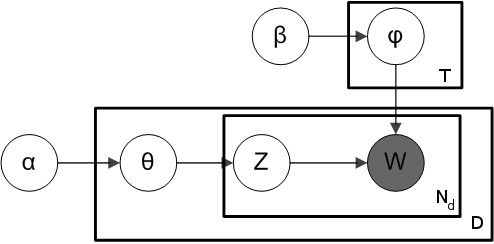
\includegraphics[width=3in]{lda-diagram.png}  %[height=1in,width=1in,angle=-90]{foo}
    \caption{ The graphical model behind LDA. $\theta$ is the distribution  of topics for a document,
              $\beta$ is the distribution of words for a given topic.}
    \end{center}
    \end{figure}


\section{The inference algorithm}

    First we being by defining some quantities
    
    We have the document set $\DD = \{ d_1, d_2, \ldots, d_D \}$, where each document consists of 
    a word count vector for the words taken from a fixed vocabulary $\WW$ of size $W$.
    
    Our aim is to produce a set of topics $\TT$ where each topic is a probability distribution over words $\WW$.
    
    
    \begin{description}
	\item[$\gamma_{wjk}$:]	$=Pr( z=k | x=w,d=j)$, the probability that word $w$ in document $j$ 
						is assigned to the topic k.
	\item[$N_{wj}$:]	\# of times $w$ appears in doc $j$. 
	\item[$N_{wk}$:]  $=\displaystyle\sum_{j\in \DD} N_{wj}\gamma_{wjk} = $ \# of times $w$ appears in topic $k$.
	\item[$N_{kj}$:]  $=\displaystyle\sum_{w\in \WW} N_{wj}\gamma_{wjk} = $ \# of times topic $k$ appears in doc $j$.
	\item[$N_{k}$:]  $=\displaystyle\sum_{w\in \WW} N_{wk}=  \displaystyle\sum_{w\in \WW}\sum_{j\in \DD} N_{wj}\gamma_{wjk} $ \# words assigned to  topic $k$.
	\item[$N_{j}$: ]  $=\displaystyle\sum_{k \in \TT} N_{kj} =  \displaystyle\sum_{k \in \TT}\sum_{w\in \WW}N_{wj}\gamma_{wjk} $ \# words in doc $j$.
    \end{description}


    To achieve this we will have to learn...


\section{The data set} \label{section:data-set}

	The good people who run the arXiv.org were kind enough to send me the entire collection of papers
	in the \texttt{quant-ph} repository! 
    The arXiv is a prominent publication in the physical sciences and contains pre-print versions
    of most of the important research in several areas.
    Of particular interest is the field of quantum information science which is very well
    represented.
	
    The raw data that was received consists of two directories. 
    The first directory, \file{pdf/} of size 7.1GB contains 31739 pdf documents.
    The second directory \file{tex/}  contains the \LaTeX \ source code of some of the papers 
    (its size is 2.1G and it contains 21061 files). 
    Since the source code of only about $2/3$ of the papers was available, we decided to use 
    the pdf version of the document collection.

    %	\begin{verbatim}
    %	ivan@flicker:/scratch/arxiv$ du -sh *
    %	7.1G    pdf
    %	2.1G    tex
    %	ivan@flicker:/scratch/arxiv$ find pdf/ -type f | wc
    %	31739   31739  730019
    %	ivan@flicker:/scratch/arxiv$ find tex/ -type f | wc
    %	21061   21061  470945
    %	\end{verbatim}
        
    %	The \texttt{pdf/} directory contains the pdf versions of the papers and for some of these papers.
    %	For about $2/3$ of these we also have the latex source code in the \texttt{tex/} directory.
        
	Some more information about the raw dataset.
	\begin{itemize}
		\item Total number of pdf files: 31739
        \item Total number of papers: 20166 (multiple versions v1,v2)
        \item Number of files with unreadable/foreign fonts: 6
		\item Earliest date: 22 Dec 1994  (pdf/9412/9412002v1.pdf)
		\item Most recent:  30 Mar 2007 (pdf/0703/0703278v1.pdf)
	\end{itemize}
	
	
	
	\subsection{Textual pre-processing}

        Since the intended feature vectors are word counts, we used the command-line utility
        \texttt{pdftotext} (part of \program{xpdf}) to convert the pdf documents to text files.
        The python script \file{preprocessing/pdftotext.py} accomplishes this and stores the
        output in the folder \file{data/text} while at the same time creating an inventory of
        all the available documents.
        At this stage, some documents were found to be unreadable or used foreign language fonts
        which were not recognized by xpdf. There were very few such documents so it was possible
        to manually remove them from the inventory.

        At this point we had 31732 documents in our ``inventory'', but some of these documents
        were different version of the same underlying paper (ex: \file{9412002v1.pdf},
        \file{9412002v2.pdf}, etc.).
        We therefore ran \program{dupremover.py} which kept only the latest version.
        After this step, the total number of papers in our data set decreased to 20166.

        Before we can perform any word counts, however, we had to deal with a typographical issue.
        Ligatures are linkages between the letters f, l and i in high quality fonts.
        Since \LaTeX \ uses the computer modern fonts which have ligatures, the document collection
        was full of them. For example, when I write the word ``affluent'' it will not be translated
        into the sequence of characters a,f,f,l,u,e,n,t but instead turn into a,ffl,u,e,n,t where 
        ffl is a single Unicode character. Can you see the difference between ffl and f{}f{}l?
        In order to deal with this issue, I did a preliminary pass using \program{makewordstream.py}
        expanding all ligatures to their constituent letters. 
        While I was at it, I also converted all words to lowercase ASCII.
		  

    \subsection{Dictionary selection}

        The next step was to select a subset of all the words that occur in the document collection
        for which we will perform word count.
		I first pass was made on the documents to remove a standard list of stopwords (see
        \file{stopwords.py}). 
		Given how large the dataset is we did not feel it was necessary to use word stemming;
        this way we can capture as much of the granularity of the data as possible.

        The total number of unique words of 3 character or more at this step was 67075, and
        contained lots of non-words like ``ijk'', which probably refer to matrix indices.
        While 60k words is not an unreasonable dictionary size, it was deemed too large for
        our purposes and an effort was made to cut down on the dictionary size.
        The script \program{makevocab.py} goes through the word stream and counts total
        number of occurrences for each word. It then rejects all words that occur less than
        45 times in the corpus. 
        We also impose a minimum occurrence threshold of 10000, 6000 and 2000 for three, four and
        five letter words respectively.

        The final pre-processing step selects the top 10011 words by overall frequency 
        and stores it in the file \file{vocab.txt}.
        This figure was inspired by the paper \cite{Blei2009}, where they use a vocabulary of this
        size on a document collection roughly similar to our own.


    \subsection{Sparse matrix format}

        The input data that the \program{topicmodel} program expects is in a standard sparse 
        matrix format which is generated by the script \program{Makedocword.pl}.
        The resulting file \file{docword.txt} contains one row for each unique word
        in each document. For example, consider the following excerpt:
        \begin{verbatim}
        #docword.txt
        ...
        34 376 6
        34 6767 5
        ...
        \end{verbatim}
        These two lines indicate that the document with id=34 contains 6 occurrences of word 376
        and 5 occurrences of word 6767.
        This is the standard bag-of-words paradigm for each document.
        %    folder + symlinks\\


    The following list summarizes the important details of the finalized data set 
    at the stage when it is read to be fed to the Gibbs sampling inference algorithm.
	\begin{itemize}
        \item Size of vocabulary: $W=10011$  
        \item Total number of documents: $D=20166$ 
        \item Total number of words in corpus: $N=41202148$
          %\item Total number of unique words: $N=11220266$
	\end{itemize}



\section{Results} \label{section:results}


    Using the above data set we perfomed a number of runs and recorded the resulting
    topics and other parameter like runtime and memory usage. 
    We report on our finding in this section.


    \subsection{Evaluation of extracted topics}

        The natural application of topic models is the automated extraction of topics from
        the data set.
        Given that we have learned the probability family of distributions $\varphi_{tw}$,
        we can now query it to see what are the most common words for each topic.
        The results of a test run with $T=20$ topics and $NITER=300$ iterations of the Gibbs chain
        are displayed in Table \ref{table:topics} on page \pageref{table:topics}.

        Everytime I ran the algorithm, I was surprized by its amazing power to pick out clusters
        of words that belong togher. 
        I discussed the words for each topic with some colleagues and they were also amazed at
        the accuracy of the produced clusters.
	

        \begin{table}
        \centering
        \caption{Automatically extracted topics.}
        \vspace{0.05in}
        \begin{footnotesize}
        \begin{raggedright}
        \begin{tabular}{|p{4.7in} p{1.2in} |}
        \hline \rule{0pt}{3ex}
        Common words in topic           & my labelling \\[3pt]
        \hline \rule{0pt}{3ex}
        (t1) quantum theory mechanics physical classical physics interpretation probability time state space
        possible principle fact point description properties question sense probabilities ...
        & general QM \\

        (t2) entanglement states state entangled phys rev pure local lett mixed separable quant systems
        maximally bipartite measure horodecki concurrence schmidt ghz ...
        & entanglement \\
        (t3) let theorem set proof follows definition lemma positive case define section defined prove
        exists consider condition implies holds map finite ...
        & math jargon \\

        (t4) quantum algorithm problem number probability classical log time computation complexity graph
        computer algorithms random function polynomial search input problems step ...
        & computing \\
        (t11) qubit quantum state qubits gate gates control operation computation operations single unitary
        circuit controlled computer fig universal states implementation sequence ...
        & computing 2 \\

        (t5) state states coherent phys mode rev noise number quantum gaussian modes field squeezing
        squeezed function vacuum lett phase operator exp ...
        & optics \\
        (t8) photon photons beam single polarization signal detection fig optical detector interference
        light rev experimental phys lett experiment source detectors pump ...
        & optics 2 \\

        (t6) measurement quantum measurements state bell probability particle local inequality experiment
        phys observables observable measured correlations particles probabilities measuring non inequalities
        ...
        & Bell inequalities \\

        (t7) space quantum group representation algebra operators operator hilbert invariant theory
        structure defined lie dimensional classical functions product vector form representations ...
        & algebra \\

        (t9) spin hamiltonian phys energy state model rev interaction ground magnetic states coupling spins
        lett systems quantum lattice electron field interactions ...
        & physics \\
        (t15) atom field atoms cavity atomic state frequency laser rev level phys transition coupling
        resonance interaction pulse trap fig optical ion ...
        & atomic phys \\
        (t16) equation function potential phys solution functions equations energy solutions form order
        hamiltonian exp integral schrdinger problem case real oscillator terms ...
        & schrodinger \\
        (t18) time quantum evolution initial classical dynamics decoherence equation environment systems
        phys hamiltonian density stochastic process decay dynamical model interaction state ...
        & decoherence \\
        (t10) error quantum code errors codes correction noise qubits encoded encoding block number level
        stabilizer fault probability rate pauli threshold measurement ...
        & error correction \\

        (t12) wave particle field energy momentum particles time force mass function phys scattering motion
        free relativistic position theory velocity fields effect ...
        & field theory \\
        (t13) phase cos sin exp case function phys momentum distribution angle initial obtain wigner
        geometric classical phases angular axis consider rotation ...
        & particle physics \\

        (t14) fig results values line figure large small case numerical number shown parameters order
        parameter region obtained function shows limit average ...
        & science jargon \\


        (t17) matrix operator operators states basis density matrices form vector unitary elements state set
        vectors product case diagonal eigenvalues terms orthogonal ...
        & linear algebra \\
        (t19) alice bob quantum protocol key communication information classical state bit teleportation
        scheme eve protocols bits basis security bobs channel alices ...
        & crypto \\
        (t20) information quantum state states entropy optimal channel fidelity probability log measurement
        classical input channels pure output cloning ensemble capacity povm ...
        & information theory \\

        %Coating thickness that attenuates cell traction force microscopy measurements by a certain
        %percentage & Independent $\left(\propto r\right)$\\[3pt]
        %Coating thickness that maintains a certain cell behavior & Increase\\[3pt]
        \hline
        \end{tabular}
        \label{table:topics}
        \end{raggedright}
        \end{footnotesize}
        \end{table} 


    \subsection{Number of topics}

        Another factor that needs to be investigated is how the performance of the algorithm
        varies when different number of topics are sought.
        We ran a series of experiments with $NITER=100$ and different values of $T$ randing
        from 3 to 200.

        During the entire test sequence, the memory consumption remained roughtly constant
        and for all experiments the memory used was roughly 700MB.
        The running time increased linearly with the number of topics as can be seen from
        Table \ref{table:runtimeT} below.

        \begin{table}[htb]
        \centering
        \caption{Runtime as a function of number of topics.}
        \begin{tabular}{|r r|}
        \hline
        T   &   runtime (s) \\
        \hline
            3 &  1447 \\
            5 &  1650 \\
            10 &  2079 \\
            15 &  2538 \\
            20 &  2857 \\
            25 &  3248 \\
            30 &  3601 \\
            40 &  4230 \\
            50 &  4924 \\
            75 &  6610 \\
            100 &  8130 \\
            150 &  11183 \\
            200 &  14167 \\
        \hline
        \end{tabular}
        \label{table:runtimeT}
        \end{table} 
        



    \subsection{Gibbs sampling chain length}

        The other parameter we chose to vary in our experiments was the length of
        the chain which we use for Gibbs sampling. 
        We held the number of topics constant at $T=20$ and varied the number
        of iterations from 5 (which would certainly be insufficient) to 300 which
        is probably overkill.

        The running time results are shown in Table \ref{table:runtimeNITER}.
        The fact that the runtime increases linearly with $NITER$ should come
        as no surprize since $NITER$ is simply the maximum value of the outermost loop
        in the Gibbs sampling routine.

        \begin{table}
        \centering
        \caption{Runtime as a function of length of Gibbs sampling.}
        \begin{tabular}{|r r |}
        \hline
        NITER   &   runtime (s) \\
        \hline
               5&         229 \\
              10&         407 \\
              20&         768 \\
              30&        1138 \\
              50&        1861 \\
              75&        2772 \\
             100&        3742 \\
             150&        5535 \\
             200&        7424 \\
             300&       10993 \\
        \hline
        \end{tabular}
        \label{table:runtimeNITER}
        \end{table} 
        
        The real data which we intended to collect in order to evaluate these runs 
        is the perplexity and not the runtime.
        

    \subsection{Perplexity}

        A quantitative method for evaluating the performance of a topic model 
        is to calculate the perplexity of the document set given the learned parameters.

        \begin{equation}
            pplex\!\left(\DD\right) = \exp\left( - \frac{1}{N} \sum_1^N \log P(w_n|d_n) \right) =
            \exp\left( - \frac{1}{N} \sum_{j=1}^D\sum_{w=1}^W N_{wj}\log P(w|d) \right) ,
        \end{equation}

        The perplexity is a measure of how ``surprized'' the model is to observe the data $\DD$.


        I wrote a program \program{perplexity.py} which can compute the perplexity of the data set
        given the topic-word distribtion $\varphi$ and the document-topic distribution $\theta$.
        {\bf Unfortunately}, by the time the moment came to evaluate the data from the various test
        runs I had been performing over the past couple of days I realized that my script had 
        a major bug in it.
        The output of each run was overwriting the output of the previous run!

        Thus I am forced to give anecdotal calculations of the perplexity based on the last run
        of each experiment. 
        \begin{itemize}
            \item For $NITER=300$, and $T=20$ we had $pplex=1349.88$
            \item For $NITER=100$, and $T=200$ we had $pplex=952.31$
        \end{itemize}

        Despite having so little data, we can observe two interesting facts. 
        First, the more topics we have the better the 

        To be honest, I must note that my perplexity calculation above may be misleading since
        it uses the same data for both training and testing. 
        It is conceivable that the model might be overfitting specific patterns in the training
        set and decrease the inbred-test perplexity while at the same time have a poor
        generalization performace.
        The correct approach would be to separate a portion of the data and use it as a test set
        according to the detailed procedures outlined in \cite{heinrich2005parameter}.
        


	
	
\section{Discussion and Conclusion}

    This project has been a very good opportunity to learn about LDA and machine learning in
    general.
    I learned both theoretical facts about graphical models as well as practical consideraitons
    about programming inference algorithms, memory management and data pre-processing.

    While I was able to extract reasonably good topics from the \texttt{quant-ph} archive,
    I think there is still a lot of left of interesting experiments to perform with this data set.
    In particular I would like to use the extracted topics in order to devlop an automated
    recommendation system or a ``topic filter'' which would help me keep track of which papers
    are posted on the arXiv every day that are relevant to my topics of research.

    Some other ideas that I would like to pursue are the following.

	\subsection{Regular expressions counts}
        
        In text analysis we invariably use word counts as the main ``features'' of documents.
        Since we have the full power and flexibility of python during the pre-processing state,
        we could use instead regular expressions as additional features.

        For example we could quantify how many matches to the reg ex \texttt{H(.*)} there are
        in each document. Certainly, for papers that deal with information theory this will be 
        a highly informative feature.

		%We can have higher level features counts from regular expression matches.
		%These features can themselves be refined over generations or by cross validation.
		%Come to think of it you can do all kinds of things with this.
        Another possible use of regular expressions is to have a digram model with synonyms
        taken into account. For example we could count how many matches there are to this
        reglar expression \texttt{quantum (mechanics|physics)} instead of trying to keep
        track of the two options separately.
		
		%Algorithm: Self-refining regular expression features
		%\begin{enumerate}
		%	\item	Start with word counts for a fixed list of words of size $|W|$ and do regular LDA.
		%	\item	For each of the latent topics build all "two word" combinations.
		%	\item	Rerun LDA on the expanded feature space of size $|W|^2 + |W|$.
		%	\item	Find the important second order occurrences and discard all other features.
		%	\item	Try to compress multiple variations using regular expression language. \\
		%			Example: "a b", "a c", "a d"  can be converted into regex "a (b|c|d)"
		%	\item	Go to step 3 but now number of features is $|W|+$ n\_of\_good\_reg\_exes
		%\end{enumerate}

		%I am not sure if this will generate all possible word occurrences but I think reg-exes are
		%pretty rich as feature set and their computation is all parallelizable so it doesn't matter if 
		%it is very expensive.
		
		%Can we let some genetic algorithm work on this instead?


    \subsection{Two data set correlations}

        I have not seen in the litterature any discussion about using LDA to automatically
        create links between two data collections.
        For example if we trained a topic model on wikipedia articles and the arXiv,
        we would be able to automatically generate meaningful links between the two.
        As you browse the arXiv you get suggested articles on wikipedia that cover similar topics.

	
	%\subsection{This paper covers}
	%
	%	User interface idea: papers laid out on a table in such a way that the papers that
	%	cite each other overlap. All papers in the same "epoch" are visible at the same time
	%	and placement and paper size indicates relative importance.
	%	
	%	(One way to think about this is where are the words of this each topic passed on from one generation
	%	to the next)
		
	\subsection{Parallel LDA}

        One aspect that I did not get a chance to look into deeper is the use of parallel algorithms
        for inference of the LDA model.
        One approach is to modify the Gibbs sampling or variational methods to permit loosely
        coupled parallel operation \cite{newman2006scalable,newman2007distributed}. 

        Another approach is to use GPU based computation which is highly parallel and vectorized.
        CUDA (Compute Unified Device Architecture) is a simple API which allows for GPU programming
        on NVIDIA grpahics boards. The speedups reported are very impressive
        \cite{masada2009accelerating, yan-parallel}.
        This research direciton would also be an excuse for me to buy an expensive graphics card.

			
    \subsection{Citation graph}

        One simple further step that can be taken to make use of the arXiv topic model 
        is to extract the citation graph amongst the paper. This can be done with another
        regular expression of the form \texttt{quant-?ph\\d\{7\}} or from some third party
        source like Citeseer.
        
        Having the citaiton graph would allows us to do a ``page rank'' type of calculation
        and extract a sense of importance for the papers in each topic.


%    \section{Metadata}
%        We should have the titles for each of these articles I think
%        we need a little urllib2 script to get each of
%        \verb|http://arxiv.org/list/quant-ph/0003?show=1000|
%        where 0003 corresponds to my folder 0003 


    Calculate perplexity and KL distance for different runs with same parameters
    \cite{newman2006scalable}.




\bibliographystyle{alpha}
\bibliography{arXivLDA}


\end{document}
